\problemname{Fire Hydrant}

Fireman Robert has been working as a firefighter for over 20 years and loves his job.
After a long walk in the metropolis M (formerly known as Stockholm), Robert received
a call on his phone from his hydrophobic boss, ordering him to come to the fire station immediately.

Robert has just arrived at the southwest intersection of the metropolis M and
decides to head straight to the fire station. However, several fire hydrants in
the metropolis M have started leaking water and flooding the streets. Oh no! This
is particularly serious because Robert's hydrophobic boss at the fire station is strict
about not having water nearby. Showing up soaking wet to work after encountering
several leaking fire hydrants could get Robert fired. Robert wants to work as a
firefighter for at least another 20 years, so please help Robert minimize how wet he gets!

Metropolis M consists of a grid of intersections with dimensions $W \times H$, where
each intersection can be reached from the four adjacent intersections in each cardinal
direction: north, east, south, and west. Robert has just arrived at the intersection
located at $(1,1)$. He wants to reach the fire station at the northeast intersection,
located at $(W,H)$. It takes exactly 1 minute to run from one intersection to another
adjacent intersection.

Furthermore, there are $N$ intersections with a leaking fire hydrant, which can be
located at any intersection in the grid, including where Robert starts at $(1,1)$
and at the fire station $(W,H)$. Robert arrives at intersection $(1,1)$ at time 0,
and each leaking fire hydrant leaks one unit of water into the intersection it is at.
But for each minute $t$ that passes, each leaking fire hydrant will leak an additional
unit of water to all intersections within the Manhattan distance $t$ from that 
eaking hydrant. Let's call the number of water units at a specific intersection $v_t$
at time $t$. When Robert arrives at an intersection at time $t$, his clothes will get
wet from all the water at that intersection due to leaking hydrants, i.e., $v_t$ water units.

What is the minimum number of water units that Robert's clothes can get wet from on his way to the fire station?


\begin{centering}
  \begin{figure}[h]
    \centering
  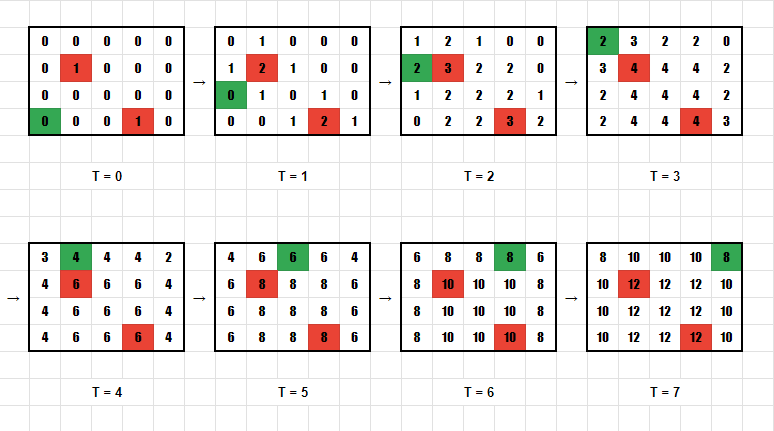
\includegraphics[width=0.8\textwidth]{brandpostSample1.png}
    \caption{Illustration of sample 1, where the green square is Roberts position and the
    red squares are the positions of the fire hydrants. The smallest total water units
    Bob can have when arriving at the station is $0+0+2+2+4+6+8+8=30$.}
    \label{fig:brandpost}
  \end{figure}
\end{centering}

\section*{Input}
The first line of the input contains three integers $W,H,N$ ($1 \le W,H \le 1000$, $1 \le min(20000,W \cdot H)$), 
where $W$ and $H$ are the width and height of the grid and $N$ is the number of leaking fire hydrants.

The following n rows each contain two integers $x_i$ and $y_i$ ($1 \le x_i \le W$, $1 \le y_i \le H$),
where $(x_i,y_i)$ is the position of the $i$:th leaking fire hydrant. It is guaranteed that no two
fire hydrants occupy the same position.

\section*{Output}
Print an integer, the least number of water units Robert can have after he arrives
at the station.

\section*{Points}
Your solution will be tested on several test case groups.
To get the points for a group, it must pass all the test cases in the group.

\noindent
\begin{tabular}{| l | l | p{12cm} |}
  \hline
  \textbf{Group} & \textbf{Point value} & \textbf{Constraints} \\ \hline
  $1$    & $10$       & $W,H \le 10$, $N=1$ and the only fire hydrant is located at $(1,1)$ \\ \hline
  $2$    & $15$       & $W,H,N \le 50$ \\ \hline
  $3$    & $17$       & $W,H \le 100$, $N\le 200$\\ \hline
  $4$    & $27$       & $W,H \le 150$ \\ \hline
  $5$    & $31$       & No additional constraints. \\ \hline
\end{tabular}
